% !TEX root = ../main.tex
\chapter{Implementation Details}
%\section{Detailed Validation Results}
\label{chapter:DetailedDescriptions}\label{appendix}
%\inputminted{c++}{../../src/wos_native.cuh}

\chapter{Meta World}
\label{chapter:MetaWorld}\label{appendix}

\chapter{Additional Plots}

\begin{figure}[htbp]
    \centering
    \begin{subfigure}[b]{0.45\textwidth}
      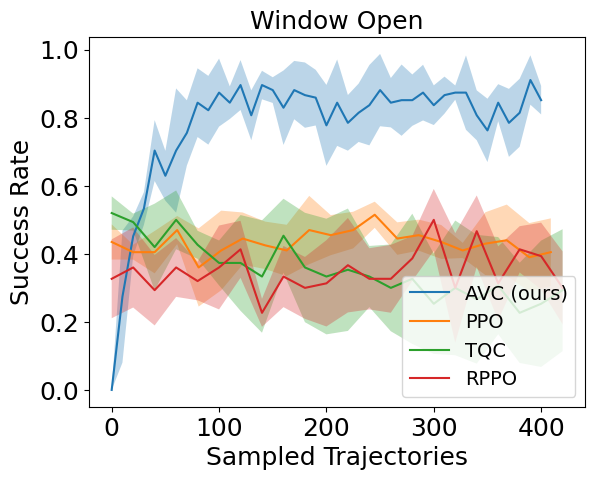
\includegraphics[width=\textwidth]{images/4_400/Window Open.png}
      \caption{Window Open environment.}
      \label{fig:plot1}
    \end{subfigure}
    \hfill
    \begin{subfigure}[b]{0.45\textwidth}
      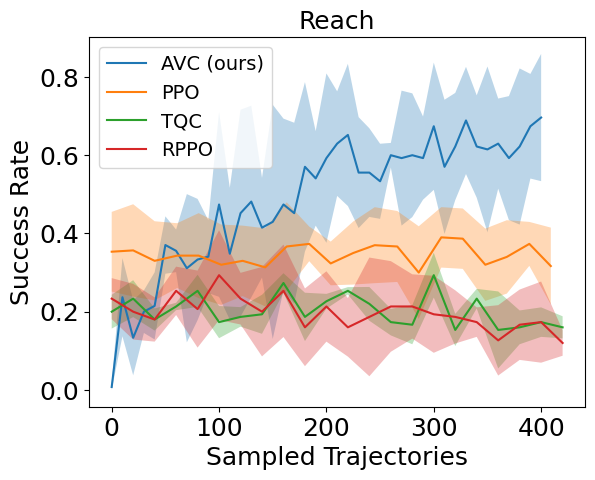
\includegraphics[width=\textwidth]{images/4_400/Reach.png}
      \caption{Reach environment.}
      \label{fig:plot2}
    \end{subfigure}
    \medskip
    \begin{subfigure}[b]{0.45\textwidth}
      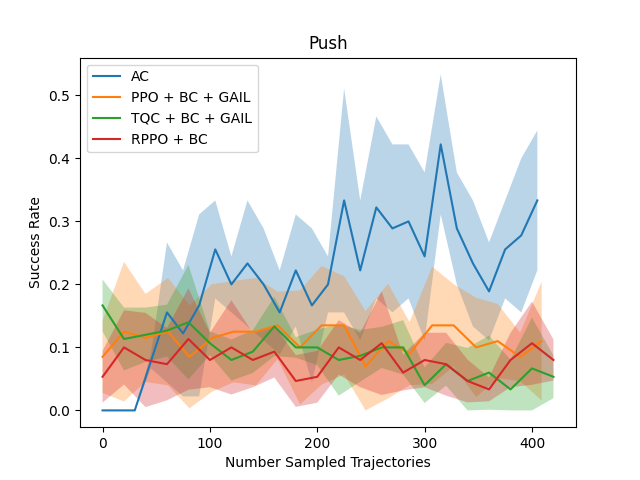
\includegraphics[width=\textwidth]{images/4_400/Push.png}
      \caption{Push environment.}
      \label{fig:plot3}
    \end{subfigure}
    \hfill
    \begin{subfigure}[b]{0.45\textwidth}
      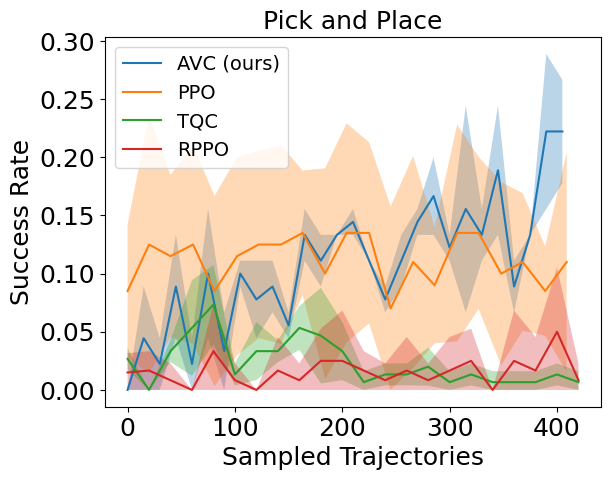
\includegraphics[width=\textwidth]{images/4_400/Pick and Place.png}
      \caption{Pick and Place environment.}
      \label{fig:plot4}
    \end{subfigure}
    \caption{Each learner had access to 4 expert demonstrations. 
    The learner trained by GAIL and RPPO were pretrained using behavioural cloning given the 4 demonstrations. 
    The x-axis shows the number of sampled environment epsiodes, each with 100 steps. One initial observation and a sparse reward signal at the end of each episode was provided.}
    \label{fig:4}
\end{figure}

\begin{figure}[htbp]
    \centering
    \begin{subfigure}[b]{0.45\textwidth}
      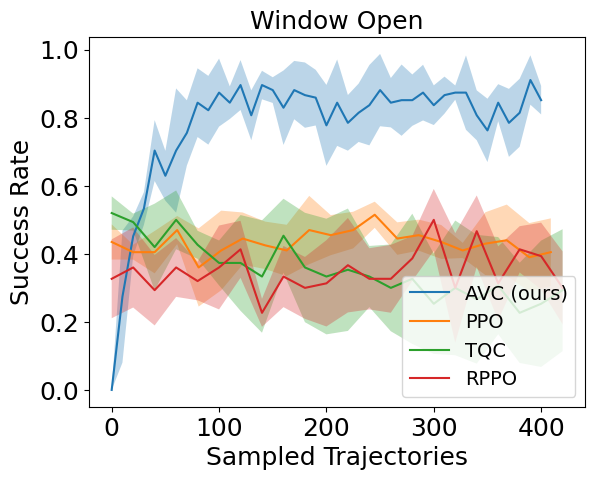
\includegraphics[width=\textwidth]{images/4_400/Window Open.png}
      \caption{Window Open environment.}
      \label{fig:plot1}
    \end{subfigure}
    \hfill
    \begin{subfigure}[b]{0.45\textwidth}
      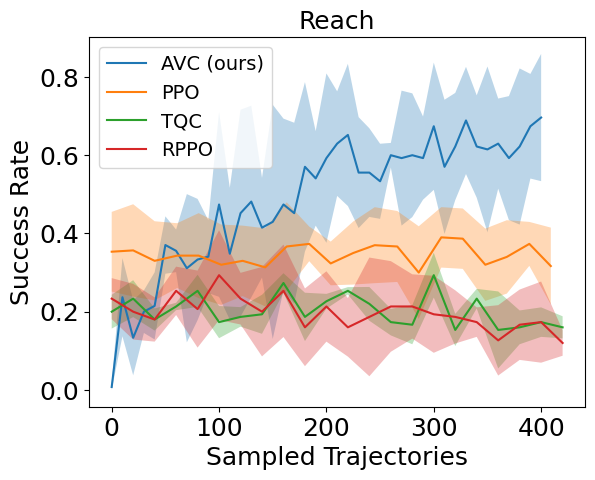
\includegraphics[width=\textwidth]{images/4_400/Reach.png}
      \caption{Reach environment.}
      \label{fig:plot2}
    \end{subfigure}
    \medskip
    \begin{subfigure}[b]{0.45\textwidth}
      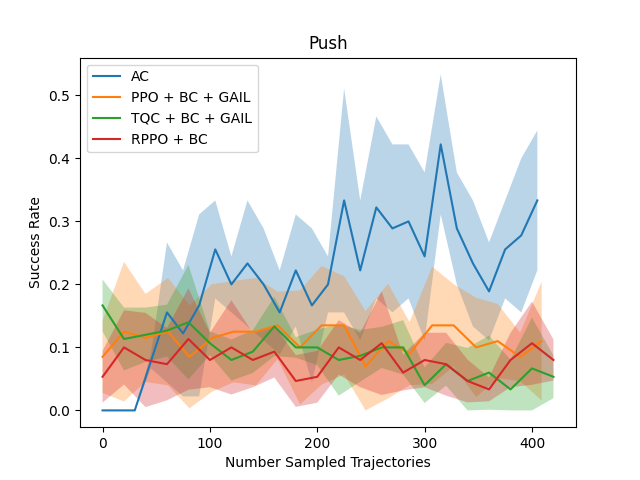
\includegraphics[width=\textwidth]{images/4_400/Push.png}
      \caption{Push environment.}
      \label{fig:plot3}
    \end{subfigure}
    \hfill
    \begin{subfigure}[b]{0.45\textwidth}
      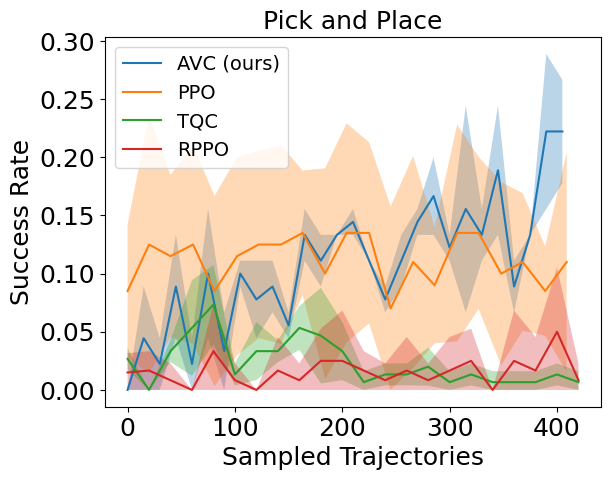
\includegraphics[width=\textwidth]{images/4_400/Pick and Place.png}
      \caption{Pick and Place environment.}
      \label{fig:plot4}
    \end{subfigure}
    \caption{Each learner had access to 4 expert demonstrations. 
    The learner trained by GAIL and RPPO were pretrained using behavioural cloning given the 4 demonstrations. 
    The x-axis shows the number of sampled environment epsiodes, each with 100 steps. One initial observation and a sparse reward signal at the end of each episode was provided.}
    \label{fig:4}
\end{figure}